\documentclass[a4paper,10pt]{article}
%\usepackage{fullpage}
\usepackage{amsmath}
\usepackage{amssymb}
\usepackage{booktabs}
\usepackage{color}
\usepackage{graphicx}
\usepackage{hyperref}
\usepackage[utf8]{inputenc}
\usepackage{listings}
\usepackage{pdfpages}
\usepackage{tabularx}
\usepackage{url}

% style customization
\definecolor{ilcodebg}{rgb}{0.95,0.95,0.95}
\definecolor{lstcomment}{rgb}{0.0,0.5,0.0}
\definecolor{lstkeyword}{rgb}{0.0,0.0,0.75}
\lstset{%
  backgroundcolor=\color{ilcodebg},
  basicstyle=\footnotesize,
  breakatwhitespace=false,
  breaklines=true,
  captionpos=b,
  commentstyle=\color{lstcomment},
  frame=single,
  keepspaces=true,
  keywordstyle=\bf\color{lstkeyword},
  language=C,
}
\newcommand{\tabref}[1]{Table~\ref{#1}}
\newcommand{\figref}[1]{Figure~\ref{#1}}
\newcommand{\lstref}[1]{Listing~\ref{#1}}
\newcommand{\ilcode}[1]{\begingroup
	\setlength{\fboxsep}{1pt}\colorbox{ilcodebg}{\small\tt%
		#1%
	}\endgroup}

\title{R2DAQ\\{\Large ROACH2 Digital Acquisition System\\for Project~8 Phase~II}}
\author{Andr\'e Young\\\url{andre.young@cfa.harvard.edu}}
\date{\today}

\begin{document}

\maketitle 

\section*{About this document}
This document describes the digital acquisition system developed for 
Project~8 Phase~II on the ROACH2 platform.

\section*{Document history}
\begin{tabularx}{1.0\textwidth}{|r|l|l|X|}
	\hline
	{\bf Version} & {\bf Date} & {\bf Authors} & {\bf Summary of changes}\\
	\hline
	1.00 & \today & AY & Initial version\\
	\hline
\end{tabularx}

\tableofcontents{}
\listoffigures{}
\listoftables

\section{Hardware}
\label{sec:hardware}
General information on the ROACH2 platform and related topics is 
available from the CASPER~\cite{casperroach2}. The purpose of this section is 
to specify the exact hardware make-up that comprise the system in-use.

A summary of the build specifications of the ROACH2 appears in 
\tabref{tab:r2build}. More detailed information can be found in the 
assembly notes in Appendix~\ref{sec:r2assy}.

\begin{table}[h]
	\centering
	\begin{tabular}{lp{0.7\textwidth}}
		{\bf Component} & {\bf Comments}\\
		\midrule
		FPGA & Xilinx Virtex6 XC6VSX475T-1FFG1759C\\
		\midrule
		ADC  & \parbox[t]{0.7\textwidth}{
					2$\times$ ASIAA 5~GSps ADC~\cite{casperadc}\\
					DMUX 1:1 version (8-bit resolution)}\\
		\midrule
		Network & \parbox[t]{0.7\textwidth}{
					2$\times$ Quad-SFP+ mezzanine~\cite{caspersfp}\\
					8$\times$ 10~Gbps total datarate}\\
		\midrule
		Enclosure & 1U mechanical enclosure\textsuperscript{*}\\
		\midrule
		Misc & \parbox[t]{0.7\textwidth}{
					ROACH2 rev.2 JP2 shunted\textsuperscript{*} (autostart on AC power)\\
					6~dB attenuator on each ADC I input\textsuperscript{*}\\
					Clock split internally to each ADC\textsuperscript{*}}\\
		\hline
		\midrule
		\multicolumn{2}{l}{\textsuperscript{*}\footnotesize{
			See Appendix~\ref{sec:r2assy}.}}
	\end{tabular}
	\caption{ROACH2 build specifications.}
	\label{tab:r2build}
\end{table}

\figref{fig:r2front} and \figref{fig:r2rear} show the front and rear 
panels, respectively, on the ROACH2.

\begin{figure}[h]
	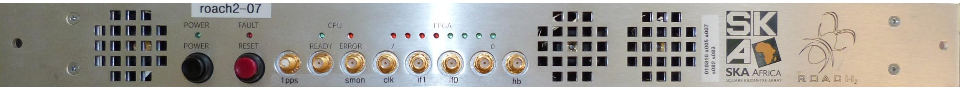
\includegraphics[width=\textwidth]{./roach2-front.png}
	\caption{ROACH2 front panel.}
	\label{fig:r2front}
\end{figure}

\begin{figure}[h]
	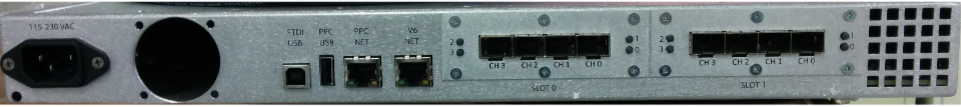
\includegraphics[width=\textwidth]{./roach2-rear.png}
	\caption{ROACH2 rear panel.}
	\label{fig:r2rear}
\end{figure}

\section{Installation}
\label{sec:installation}
This section describes the steps required to configure and install a 
new ROACH2 system on a Linux server (assuming Debian-like distribution).
The steps covered include:
\begin{enumerate}
	\item configuring ROACH2 to boot from network using DHCP and NFS,
	\item configuring the Linux server to provide the necessary services,
	\item install software needed to interface with and program the ROACH2, and
	\item cable setup of the ROACH2.
\end{enumerate}

\subsection{ROACH2 configuration}
\label{sec:r2conf}
This section is a customized summary\footnote{Credit to Laura 
Vertatschitsch for creating a first version of this set of 
instructions.} of the notes in~\cite{caspernfs}.

\begin{enumerate}
	\item Connect the ROACH2 to AC and power it up (if this does not 
	happen automatically).
	\item Connect a USB type-A to type-B cable between the ROACH2 (the
	port labeled ``FTDI USB'') and the Linux server. The USB interface
	will show up as four serial devices under \ilcode{/dev/ttyUSB*}, 
	the third one is usually the right one to connect to (typically 
	\ilcode{dev/ttyUSB2}). You can also use \ilcode{lsusb} to help 
	identify the correct USB device; look for {\bf Future 
	Technology Devices International, Ltd FT4232H Quad HS USB-UART/FIFO 
	IC}.
	\item As root, do \ilcode{screen /dev/ttyUSB2 115200} (or whatever
	you have identified as the correct USB device) which will connect to 
	the device terminal. At this point you want to do a soft reset of 
	the ROACH2, and how to do that depends on how it was last configured.
	\begin{enumerate}
		\item If you are faced with a login prompt it likely means that 
		the system has booted from memory. Log in as \ilcode{root} 
		(blank password) and do \ilcode{shutdown -r now} to restart it.
		When the ROACH2 restarts it will give a countdown (usually 
		5~seconds) during which it allows you to interrupt the boot 
		process. Do this by pressing \ilcode{ENTER} .
		\item If you see error messages along the line of the system 
		being unable to boot, it was likely set to boot from network.
		Interrupt the process by doing \ilcode{Ctrl+c} .
	\end{enumerate}
	\item You should now arrive at a prompt, indicated by \ilcode{=>} 
	where you can verify / change the configuration of the ROACH2.
	\item Do \ilcode{printenv ethaddr} to display the MAC address of the 
	1~Gb (control network) hardware. You will need this to set up DHCP
	on the server.
	\item You can also do \ilcode{printenv} to show all environment 
	variables. Verify that the variable \ilcode{bootcmd} is set equal 
	to \ilcode{run netboot}. If it is not, do 
	\ilcode{setenv bootcmd run netboot} and then \ilcode{saveenv} to 
	set the ROACH2 to boot from the network. You can verify that the
	variable has been updated by doing another \ilcode{printenv} .
	\item Finally, do \ilcode{reset} which will restart the ROACH2, and
	if the configuration was done properly you will see it trying to 
	boot from the network. It will of course fail if the server has not 
	been configured yet to serve what the ROACH2 needs.
\end{enumerate}

\subsection{Server configuration}
\label{sec:srvconf}
The server provides to the ROACH2 its IP settings, a boot image via 
TFTP, and a filesystem for the PowerPC via NFS. It is assumed that all 
required system packages (e.g.\ \ilcode{nfs-kernel-server}, 
\ilcode{nfs-common}, etc., but which may differ among distributions) are 
installed. To set up DHCP we will use \ilcode{dnsmasq} but any other
service that offers what is needed will do.

\begin{enumerate}
	\item Identify a network interface on the server through which it
	can offer DHCP to the ROACH2. Set its IP settings to have a static 
	configuration. Bring down and back up the interface if necessary. 
	For illustration we will assume that interface \ilcode{eth1} has 
	been configured with address \ilcode{192.168.1.1} .
	\item Create the path \ilcode{/srv/roach2\_boot} .
	\item Clone \ilcode{https://github.com/sma-wideband/r2dbe.git} into 
	a temporary path. We only need the contents in the \ilcode{/support} 
	subdirectory here.
	\item Do an attribute-preserving copy of the boot image
	doing something like
	\ilcode{cp -rfp support/boot /srv/roach2\_boot} .
	\item Do an attribute-preserving copy of the tarballed filesystem by 
	doing something like
	\ilcode{cp -fp support/r2dbe-debian-fs.tar.gz /srv/roach2\_boot} .
	In \ilcode{/srv/roach2\_boot} do
	\ilcode{tar xvfz r2dbe-debian-fs.tar.gz} which will create a 
	directory called \ilcode{debian\_stable\_devel} . Rename it to 
	something like 
	\ilcode{mv debian\_stable\_devel root} .
	\item Now we are done with the cloned git repository, delete it if 
	you want to.
	\item Edit \ilcode{/etc/exports} and add the share\\
	\ilcode{/srv/roach2\_boot\ 192.168.1.0/24(rw,subtree\_check,no\_root\_squash,insecure)}
	\item Effect the changes by doing \ilcode{exportfs -r} and verify that it
	is successful by doing \ilcode{showmount -e} .
	\item Edit \ilcode{/etc/dnsmasq.conf} to include the following lines:\\
	\ilcode{\# serve an IP address, substitute the ROACH2's MAC address below}\\
	\ilcode{dhcp-host=02:44:01:02:0a:1b,192.168.1.2}\\
	\ilcode{\# serve a boot image over TFTP}\\
	\ilcode{dhcp-boot=uImage}\\
	\ilcode{enable-tftp}\\
	\ilcode{tftp-root=/srv/roach2\_boot/boot}\\
	\ilcode{\# serve root filesystem over NFS}\\
	\ilcode{dhcp-option=17,192.168.1.1:/srv/roach2\_boot/root}\\
	\ilcode{\# optional extras}\\
	\ilcode{dhcp-authoritative}\\
	\ilcode{interface=eth1}\\
	\ilcode{dhcp-range=192.168.1.128,192.168.1.255,12h}
	\item Add the ROACH2 hostname to \ilcode{/etc/hosts} by inserting 
	the line\\
	\ilcode{\# Let us call the ROACH2 by the name `led'}\\
	\ilcode{192.168.1.2 led}
	\item Restart DHCP service by \ilcode{/etc/init.d/dnsmasq restart} .
	\item Connect the ROACH2 to the network on which DHCP is served 
	through the ``PPC NET'' port, and restart the ROACH2.
\end{enumerate}

\noindent At this point the ROACH2 should try to boot over the network using DHCP 
served to it by the server. Verify that this is working by monitoring 
it through the serial interface: the output to expect will show the 
ROACH2 obtaining an IP address, successfully booting, and eventually 
displaying a login prompt. You can also monitor what the server is 
doing my monitoring various logs, for example, 
\ilcode{tail -f /var/log/syslog} during the restart.

\subsection{Software installation}
\label{sec:swinstall}
The ROACH2 should now be set up so that you can interact with it from 
the server, or any other machine that can see it on the network. You can 
log in to it via \ilcode{ssh} as \ilcode{root} and do any number of 
things that you might do on a Unix-like system. It should be running a 
service called \ilcode{tcpborphserver3} , if it is not running you can 
start it by doing \ilcode{/etc/init.d/tcpborphserver3} . (This is useful
to keep in mind for the future and is one of the things you can check 
if you have problems programming the ROACH2, which does happen, albeit 
very rarely.)

A few custom python libraries are needed to program the ROACH2 and to 
interact with it in a more targeted application. Some standard 
dependencies are needed to install these libraries and will be assumed 
to be obtainable. On the server:
\begin{enumerate}
	\item Install the KATCP protocol \ilcode{pip install katcp} . This
	is used to program the ROACH2 and to interact with the gateware. 
	\item Also do \ilcode{pip install corr} which provides wrappers to
	the functionality available in KATCP.
	\item Install the python library required to configure the ADC card 
	installed on the ROACH2. Clone it from github using\\
	\ilcode{git clone https://github.com/sma-wideband/adc\_tests.git}\\
	and in \ilcode{adc5g\_tests} do \ilcode{python setup.py install} .
	\item Clone the \ilcode{phasmid} repository using\\
	\ilcode{git clone https://github.com/project8/phasmid.git} . 
	\item Copy any gateware binaries that you intend to program from\\
	\ilcode{phasmid/casper/master/r2daq/bit\_files} to the location in the 
	mounted filesystem \ilcode{/srv/roach2\_boot/root/boffiles} 
	where the ROACH2 will be able to see it. The ROACH2 can only be 
	programmed with \ilcode{.bof} files so if you copied a zipped format 
	you will need to unzip \ilcode{gunzip bitcode.bof.gz} before 
	attempting to program the ROACH2.
\end{enumerate}

\noindent The software setup is now complete.
\subsection{Signals and cabling}
\label{sec:snc}
All that is left to do before you are able to follow the {\em Getting 
started} instructions in \ilcode{phasmid/README.md} is to provide the 
necessary analog signals and to cable up the data network. The exact 
configuration depends on the gateware version, however in general the 
following applies.
\begin{enumerate}
	\item Supply a -6~dBm 1600~MHz tone to the SMA port labelled 
	\ilcode{clk} .
	\item Provide the analog signal(s) to be digitized to the SMA port(s) 
	labelled \ilcode{if0} and/or \ilcode{if1} .
	Wideband noise at a level of -6~dBm will more or less use the full 
	range of the ADC.
	\item Connect the SFP+ cable(s) to the appropriate network port(s)
	\ilcode{CH0}--\ilcode{CH3} in \ilcode{SLOT0} and/or \ilcode{SLOT1} .
\end{enumerate}

\vspace{\baselineskip}

\noindent This concludes installation of the ROACH2 system.

\section{Gateware}
\label{sec:gateware}
This section gives an overview of the gateware design. The intention is 
more to provide the system user with a better understanding of the 
signal processing and data organization that occurs within the gateware 
than to detail the logic circuits.

The gateware can be subdivided into different groups: global status and 
control, analog-to-digital conversion, and digital channel processing. A 
description of each group is provided in the subsequent sections, 
followed by a section devoted to discussing version-specific topics.

Monitor and control of the gateware is provided through registers that
are built into the gateware and which are accessible from within the 
PowerPC, and thereby within Python through the use of the installed 
libraries. In each section devoted to a particular group of gateware 
logic the relevant input / output registers are listed and described. 
All registers are 32-bit fields and the interpretation of each are 
detailed below.

The general description below applie to the build
\ilcode{r2daq\_2016\_May\_18\_1148.bof} which is identified as version 
\ilcode{0001}. Changes in subsequent versions of the gateware are 
discussed in the section devoted to that topic.

\subsection{Global status and control}
\label{sec:gwctrl}
This group comprises mostly of time-keeping and reset logic.

A master reset signal is provided which, when triggered restores all 
subsystems to their initial state.

The time-keeping system counts the number of seconds that have passed 
since the master reset signal was last released. This value is added to 
the reference time stored in \ilcode{unix\_time0} to compute the 
current time. The reference time and current time are both 32-bit 
integers that measure Unix time, i.e.\ seconds that have elapsed since 
00:00:00 UTC on 1 January 1970.

\paragraph{Input registers}
The following input registers are associated with this group:

\subparagraph{\ilcode{master\_ctrl}}
Controls the master reset and synchronization signals.\\
\begin{tabular}{rll}
	{\bf bits} & {\bf type} & {\bf comments}\\
	0 & BOOLEAN & master reset, active high\\
	1 & BOOLEAN & manual sync, active high\\
	31..2 & n/a & not used
\end{tabular}

\subparagraph{\ilcode{unix\_time0}}
Defines the reference time.\\
\begin{tabular}{rll}
	{\bf bits} & {\bf type} & {\bf comments}\\
	31..0 & UINT\_32 & reference Unix time\\
\end{tabular}

\paragraph{Output registers}
The following output registers are associated with this group:

\subparagraph{\ilcode{master\_status}}
Copies a number of flags output from the FFT cores and packetization 
blocks. Not recommended for general use.

\subsection{Analog-to-digital conversion}
\label{sec:gwadc}
The ADC comprizes four cores that each sample the analog input in 
parallel at one quarter of the sampling rate, i.e.\ 800~MSps. By 
interleaving the cores to be 90 degrees out-of-phase with respect to 
each other, the samples can be combined to produce the sampling at 
3200~MSps. The output of the ADC is demultiplex by a factor 16 so that 
with each cycle the FPGA, which is clocked at 200~MHz is presented with 
16 consecutive time-domain samples (4 from each ADC core).

Only a single ADC, the one associated with input \ilcode{if0} and the 
\ilcode{zdok0} interface between the ADC card and the FPGA board is 
currently available in the bitcode.

\paragraph{Input registers}
n/a

\paragraph{Output registers}
n/a

\subsection{Digital channel processing}
\label{sec:gwdcp}
Three digital channels are associated with each ADC to allow for a total 
of six digital channels to be processed. That is, three digital channels 
will operate on the same data received from one particular ADC.  The 
digital channels are named \ilcode{a}--\ilcode{f}, see 
\tabref{tab:digitalchannels} for associations with each channel. Only 
channels \ilcode{a}--\ilcode{c} and FFT cores \ilcode{ab}--\ilcode{cd} 
are currently implemented.  In the following \ilcode{<x>} and 
\ilcode{<xy>} will be used as placeholders for the channel / FFT core 
designations.

Each digital channel can select a 100~MHz wide band within the 1600~MHz 
wide signal received from the ADC, and output both a time-domain and 
frequency-domain sampling of that band. The various steps in processing 
that are performed to achieve this are described in the following 
sections.

\begin{table}[h]
	\centering
	\begin{tabular}{|l|c|c|c|c|c|c|}
		\hline
		{\bf Digital channel} & \ilcode{a} & \ilcode{b} & \ilcode{c} & \ilcode{d} & \ilcode{e} & \ilcode{f}\\
		\hline
		{\bf Implemented} & yes & yes & yes & no & no & no\\
		\hline
		{\bf Digital ID} & 0 & 1 & 2 & n/a & n/a & n/a\\
		\hline
		{\bf Analog channel} & \multicolumn{3}{c|}{\ilcode{if0}} & \multicolumn{3}{c|}{\ilcode{if1}}\\
		\hline
		{\bf IF ID} & \multicolumn{3}{c|}{0} & \multicolumn{3}{c|}{n/a}\\
		\hline
		{\bf FFT core} & \multicolumn{2}{c|}{\ilcode{ab}} & \multicolumn{2}{c|}{\ilcode{cd}} & \multicolumn{2}{c|}{n/a}\\
		\hline
		{\bf SFP+ slot} & \multicolumn{3}{c|}{\ilcode{SLOT0}} & \multicolumn{3}{c|}{n/a}\\
		\hline
		{\bf SFP+ port} & \ilcode{ch0} & \ilcode{ch1} & \ilcode{ch2} & n/a & n/a & n/a\\
		\hline
	\end{tabular}
	\caption{Digital channel allocation.}
	\label{tab:digitalchannels}
\end{table}

\subsubsection{First frequency translation}
\label{sec:gwdcpddc1}
The first frequency translation mixes the 8-bit input data with a 
complex exponential to position the positive half-spectrum of the 
100~MHz wide channel-of-interest to align with an odd-numbered Nyquist 
zone for sampling at 200~Msps. The desired translation is computed in 
software (see Section~\ref{sec:software}), but is selected to be 
greater than 100~MHz in magnitude to ensure that the negative half-
spectrum of the channel is well outside the same Nyquist zone.

Sine and cosine components of the mixing frequency are generated from a 
direct digital synthesizer (DDS) implemented as a lookup table with 
10-bit phase resolution and 11-bit amplitude resolution. The given 
phase resolution is equivalent to a frequency resolution of
\begin{equation}
	\label{eq:ddc1freqres}
	\Delta_f = D F_{\text{clk}} / 2^{b_{\phi}} = 3.125~\text{MHz},
\end{equation}
where $D$ is the demux factor, $F_{\text{clk}}$ is the FPGA clock 
frequency, and $b_{\phi}$ is the phase bit-resolution.

The frequency is controlled by the register 
\ilcode{ddc\_1st\_<x>\_synth\_input\_dphi} which essentially indicates 
the phase step $\Delta_{\phi}$ between consecutive samples and thus 
determines the frequency. In order to accommodate high enough 
frequencies such that the phase may wrap within $D$ or fewer samples, 
the register also sets the phase step $D \Delta_{\phi}$ associated with 
every $D$ samples.

\paragraph{Input registers}
The following input registers are associated with this group:

\subparagraph{\ilcode{ddc\_1st\_<x>\_synth\_input\_dphi}}
Controls the DDS.\\
\begin{tabular}{rll}
	{\bf bits} & {\bf type} & {\bf comments}\\
	9..0   & UINT\_10 & common phase offset in generated sinusoid signals\\
	19..10 & UINT\_10 & number of $2\pi/2^{b_{\phi}}$ steps in phase per sample at 3200~MSps\\
	29..20 & UINT\_10 & number of $2\pi/2^{b_{\phi}}$ steps in phase per $D$ samples\\
	31..30 & n/a  & not used
\end{tabular}

\paragraph{Output registers}
n/a

\subsubsection{Bandpass filter and downsampling}
\label{sec:gwdcpddc1}
The real and imaginary components of the output of the first frequency 
translation serve as input to a 127-order finite impulse response (FIR) 
filter.
The filter output is downsampled by a factor 16 to deliver a 
time-domain digital signal at 200~MSps and a demux factor of 1.
The purpose of this filter is to suppress signal and noise 
outside the band-of-interest to a sufficient extent so as to reduce the 
impact of aliasing that results from the downsampling.
The downsampled filter output is,
\begin{equation}
	\label{eq:ddc1fir}
	y[16k\Delta_{T}] = \sum_{i=0}^{127} b_{i}x[(16k-i)\Delta_{T}].
\end{equation}

The coefficiens are real-valued and specified as 8-bit fixed-point 2's 
complement with 7 fractional bits each. Coefficients are ordered into 
groups of 4 (4$\times$8-bit = 32-bit) so that each group is associated 
with a single 32-bit register. There are 32 such registers for a single 
128-coefficient filter.

The output of the filter is multiplied by a single real-valued gain 
which is specifed as 8-bit fixed-point 2's complement with 4 fractional 
bits. The gain values for all channels are specified in the register 
\ilcode{gain\_ctrl}.

The output of the gain is split to two parallel paths, one to the STFT 
and the other to a second second frequency translation.

\paragraph{Input registers}
The following input registers are associated with this group:

\subparagraph{\ilcode{ddc\_1st\_<x>\_cb<m>\_g<n>}}
Group of four filter coefficients $\left\{b_{i}\,|\,i = 16m + 4n + j,\right.$
$\left. j = 0,1,2,3\right\}$, where $m=0,1,\ldots,8$ and $n=0,1,2,3$.\\
\begin{tabular}{rll}
	{\bf bits} & {\bf type} & {\bf comments}\\
	  7..0 & FIX\_8\_7 & 0th coefficient ($j=0$)\\
	 15..8 & FIX\_8\_7 & 1th coefficient ($j=1$)\\
	23..16 & FIX\_8\_7 & 2th coefficient ($j=2$)\\
	31..24 & FIX\_8\_7 & 3th coefficient ($j=3$)
\end{tabular}

\subparagraph{\ilcode{gain\_ctrl}}
Gain applied to FIR filter outputs.\\
\begin{tabular}{rll}
	{\bf bits} & {\bf type} & {\bf comments}\\
	  7..0 & FIX\_8\_4 & gain for channel \ilcode{a}\\
	 15..8 & FIX\_8\_4 & gain for channel \ilcode{b}\\
	23..16 & FIX\_8\_4 & gain for channel \ilcode{c}\\
	31..24 & n/a & not used
\end{tabular}

\paragraph{Output registers}
n/a

\subsubsection{Short-term Fourier transform}
\label{sec:gwdcpfft}
The STFT is computed over 8192 complex-valued time-domain samples to 
produce 8192 complex-valued spectrum samples. Since the first frequency 
translation and bandpass filter contained the band-of-interest to only 
the positive half-spectrum, only the 4096 spectrum samples that 
correspond to positive frequency are retained.

The STFT is implemented as a 13-stage FFT. There is no bit growth in the 
computation and a software-controlled shift schedule is used to avoid 
overflow. The shift schedule is a 13-bit field and the value of each bit 
determines whether the output of the associated stage should be shifted 
to the right by one position (`1') or not (`0'). A shift schedule of 
`1101010101010' ensures that overflow never occurs.

Since there are currently only two FFT cores in the design their shift 
schedules are controlled by a single register \ilcode{fft\_ctrl}.

Each FFT core has an overflow flag that indicates whether an overflow 
has occurred during the computation of the current STFT. Whenever this 
occurs a 10-bit counter associated with each FFT core increments by one. 
These counts are available in the register \ilcode{fft\_status}.

\paragraph{Input registers}
The following input registers are associated with this group:

\subparagraph{\ilcode{fft\_ctrl}}
Shift schedules for the two FFT cores.\\
\begin{tabular}{rll}
	{\bf bits} & {\bf type} & {\bf comments}\\
	  12..0 & BITFIELD & shift schedule for FFT core \ilcode{ab}\\
	 25..13 & BITFIELD & shift schedule for FFT core \ilcode{cd}
\end{tabular}

\paragraph{Output registers}
The following output registers are associated with this group:

\subparagraph{\ilcode{fft\_ctrl}}
Counts the number of overflows that have occurred per FFT core.\\
\begin{tabular}{rll}
	{\bf bits} & {\bf type} & {\bf comments}\\
	   9..0 & n/a      & not used\\
	 19..10 & UINT\_10 & overflow count for  FFT core \ilcode{cd}\\
	 29..20 & UINT\_10 & overflow count for  FFT core \ilcode{ab}\\
	 31..30 & n/a      & not used
\end{tabular}

\subsubsection{Second frequency translation and downsampling}
\label{sec:gwdcpddc2}
A second frequency translation is implemented to center the band-of-
interest, that appears only in the positive half-spectrum after the 
first downconversion, around zero. This enables the use of a low-pass 
filter with real coefficients to further suppress noise and downsample 
the time-domain signal further by a factor 2.

Since the frequency translation required here is fixed and equal to 
exactly one quarter of the sampling rate, it is efficiently implemented
as a combination of swapping real and imaginary components, and sign 
inversions.

The low-pass filter used in this stage is a 4th-order elliptic infinite 
impulse response (IIR) filter with fixed coefficients. It is implemented 
as two bi-quadratic structures, each using a scattered lookahead 
architecture with transfer function
\begin{equation}
	H(z) = \sum_{i=0}^{8} b_{i}z^{-i} \bigg/ \sum_{i=0}^{8}a_{i}z^{-i}.
\end{equation}
The coefficients for the first and second bi-quadratic structures are 
given in \tabref{tab:biquad1} and \tabref{tab:biquad2}, respectively.

\begin{table}[h]
\resizebox{\textwidth}{!}{%
	\begin{tabular}{l|r|r|r|r|r|r|r|r|r}
		$i$ & 0 & 1 & 2 & 3 & 4 & 5 & 6 & 7 & 8\\
		\hline
		$b_{i}$ & 0.81526 & 0.30303 & 0.11508 & -0.26068 & -1.00000 & -0.13922 & -0.13475 & 0.13388 & 0.40923\\
		$a_{i}$ & 1.00000 & 0.00000 & 0.00000 & 0.00000 & -1.16956 & 0.00000 & 0.00000 & 0.00000 & 0.39893
	\end{tabular}
}
	\caption{First bi-quadratic structure of elliptic low-pass filter.}
	\label{tab:biquad1}
\end{table}

\begin{table}[h]
\resizebox{\textwidth}{!}{%
	\begin{tabular}{l|r|r|r|r|r|r|r|r|r}
		$i$ & 0 & 1 & 2 & 3 & 4 & 5 & 6 & 7 & 8\\
		\hline
		$b_{i}$ & 0.67529 & 1.00000 & 0.51696 & -0.19710 & -0.12551 & -0.02349 & -0.01849 & 0.00488 & 0.00375\\
		$a_{i}$ & 1.00000 & 0.00000 & 0.00000 & 0.00000 & -0.06164 & 0.00000 & 0.00000 & 0.00000 & 0.00098
	\end{tabular}
}
	\caption{Second bi-quadratic structure of elliptic low-pass filter.}
	\label{tab:biquad2}
\end{table}

The output of the filter is downsampled by a factor two, to produce
4096 complex-valued time-domain samples in each window over which the 
STFT is computed in parallel. That is, the data rate at the downsampled 
output of the filter matches that at the output of the STFT computation.

\paragraph{Input registers}
n/a

\paragraph{Output registers}
n/a

\subsubsection{Requantization}
\label{sec:gwdcpquant}
The data at the output of each of the STFT and second downconversion is
complex-valued, and the real and imaginary components are represented as 
25-bit 2's complement fixed point with 16 fractional bits, FIX\_25\_16. 
Here the data is requantized down to 8-bit per componenent by 
reinterpreting the input data as FIX\_25\_24 and then rounding to 
FIX\_8\_7.

\paragraph{Input registers}
n/a

\paragraph{Output registers}
n/a

\subsubsection{Packetization}
\label{sec:gwdcppkt}
This block packages the time-domain and frequency-domain data produced 
after requantization for transmission over the network. Time-domain data 
and frequency-domain data are transmitted in packet pairs, where the 
first packet contains frequency-domain data over one STFT window, and 
the next packet contains time-domain data over the same STFT window.

The packet structure is defined in \lstref{lst:pkt} and contains a 
header of 32 bytes and a data payload of 8192 bytes. The interpretation 
of each header field is provided in the following.

\begin{minipage}{\linewidth}
\begin{lstlisting}[language=C,caption={Packet structure.},label={lst:pkt}]
#define PAYLOAD_SIZE 8192
typedef struct packet {
    // first 64bit word
    uint32_t unix_time;
    uint32_t pkt_in_batch:20;
    uint32_t digital_id:6;
    uint32_t if_id:6;
    // second 64bit word
    uint32_t user_data_1;
    uint32_t user_data_0;
    // third 64bit word
    uint64_t reserved_0;
    // fourth 64bit word
    uint64_t reserved_1:63;
    uint64_t freq_not_time:1;
    // payload
    int8_t data[PAYLOAD_SIZE];
} packet_t;
\end{lstlisting}
\end{minipage}

\subparagraph{\ilcode{unix\_time}} Timestamp applied to the packet in 
Unix time as seconds in 32-bit unsigned integer.

\subparagraph{\ilcode{pkt\_in\_batch}} Counts the number of packet pairs 
that have been sent within the current 16-second window. During each 16-
second window there will be exactly 390626 packet pairs, or 781252 
packets in total, sent for each digital channel. Packets within a single 
pair will have the same value for this counter.

\subparagraph{\ilcode{digital\_id}} This field indicates the digital 
channel from which the packet was sent. See \tabref{tab:digitalchannels}
for the allocation of digital identification numbers.

\subparagraph{\ilcode{if\_id}} This field indicates the analog channel 
associated with the data. See \tabref{tab:digitalchannels} for the 
allocation of analog channel identification numbers.

\subparagraph{\ilcode{user\_data\_0}} Contains the 32-bit value 
currently in the register \ilcode{pkt\_<x>\_ud0}.

\subparagraph{\ilcode{user\_data\_1}} Contains the 32-bit value 
currently in the register \ilcode{pkt\_<x>\_ud1}.

\subparagraph{\ilcode{reserved\_0}} 64-bit word not currently in use.

\subparagraph{\ilcode{reserved\_1}} 63-bit word not currently in use.

\subparagraph{\ilcode{freq\_not\_time}} Indicates whether the packet 
contains frequency-domain data (`1') or time-domain data (`0').

\vspace{\baselineskip}

\noindent Whether the packet contains time- or frequency-domain data, 
the packing order into the payload \ilcode{data} is,\\

\begin{tabular}{|c|c|c|c|c|c|c|}
	\hline
	$\textrm{im}(x_{0})$ & $\textrm{re}(x_{0})$ &
	$\textrm{im}(x_{1})$ & $\textrm{re}(x_{1})$ &
	$\cdots \qquad \cdots$ &
	$\textrm{im}(x_{K})$ & $\textrm{re}(x_{K})$\\
	\hline
\end{tabular}
\vspace{\baselineskip}

\noindent with $K=4095$, and $\textrm{re(x)}$ and $\textrm{im(x)}$ 
taking the real and imaginary components of complex-valued $x$, 
respectively. Each element in the data array may be interpreted as a 
signed 8-bit integer.

\paragraph{Input registers}
The following input registers are associated with this group:

\subparagraph{\ilcode{pkt\_<x>\_ud0}}
Specifies the 32-bit value to copy in the first user-data header field 
of packets for this channel.\\
\begin{tabular}{rll}
	{\bf bits} & {\bf type} & {\bf comments}\\
	  31..0 & BITFIELD & value to copy into \ilcode{user\_data\_0}
\end{tabular}

\subparagraph{\ilcode{pkt\_<x>\_ud1}}
Specifies the 32-bit value to copy in the second user-data header field
of packets for this channel.\\
\begin{tabular}{rll}
	{\bf bits} & {\bf type} & {\bf comments}\\
	  31..0 & BITFIELD & value to copy into \ilcode{user\_data\_1}
\end{tabular}

\paragraph{Output registers}
n/a

\subsubsection{Data transmission}
\label{sec:gwdcpdtx}
The packetized data is transmitted over high-speed network using UDP as 
the transport layer.

The transmission core for a particular digital channel is associated 
with a source IP address and port that are configured in software. In 
addition the core is assigned a MAC address and provided with an ARP 
table for all devices on the same /24 network.

The packet destination IP address and port are controlled by the 
software registers \ilcode{tengbe\_<x>\_ip} and 
\ilcode{tengbe\_<x>\_port}, respectively.

Each transmission core is also associated with a control register 
\ilcode{tenbge\_<x>\_ctrl} which provides a method by which the core 
may be reset. This may be necessary if the transmission buffer of the 
core overflows, however this is not expected to occur during normal 
operation.

One status register \ilcode{tenbge\_<x>\_status} is also associated with 
each transmission core.

\paragraph{Input registers}
The following input registers are associated with this group:

\subparagraph{\ilcode{tengbe\_<x>\_ctrl}}
Control register for the transmission core.\\
\begin{tabular}{rll}
	{\bf bits} & {\bf type} & {\bf comments}\\
	    0 & BOOLEAN & core reset, active high\\
	31..1 & n/a     & not used
\end{tabular}

\subparagraph{\ilcode{tengbe\_<x>\_ip}}
Packet destination IP address.\\
\begin{tabular}{rll}
	{\bf bits} & {\bf type} & {\bf comments}\\
	31..0 & UINT\_32     & packet destination IP address
\end{tabular}

\subparagraph{\ilcode{tengbe\_<x>\_port}}
Packet destination port.\\
\begin{tabular}{rll}
	{\bf bits} & {\bf type} & {\bf comments}\\
	 15..0 & UINT\_16     & packet destination port\\
	31..16 & n/a          & not used
\end{tabular}

\paragraph{Output registers}
n/a

\subsection{Versions}
\label{sec:gwver}
This section describes any changes to the gateware that have been 
included since the initial design described in the previous sections.

The gateware contains three registers that indicate various versioning 
information. These are \ilcode{rcs\_lib} which is associated with the 
git version control information of the CASPER library used to build the
gateware, \ilcode{rcs\_app} which is is associated with the git version 
control information of the Simulink model of the gateware design, and 
\ilcode{rcs\_app} which contains a single version number. The Python 
interface library provides a method to interpret the values of these 
registers, especially those relating to git information.

The version number in \ilcode{rcs\_app} is updated with each new build 
of the gateware, and all versions of the gateware are provided in 
\tabref{tab:masterversion}. Minor changes to the design increment the 
version number by one, and with each major change the version number is 
rounded up to the next thousand.

\begin{table}[h]
	\begin{tabular}{rl}
		{\bf Version number} & {\bf Binary file}\\
		\hline
		\ilcode{0001} & \ilcode{r2daq\_2016\_May\_18\_1148.bof}\\
		\hline
		\midrule
	\end{tabular}
	\caption{Master version table.}
	\label{tab:masterversion}
\end{table}
\vspace{\baselineskip}

\noindent Particular notes on each version are provided in the following sections. 

\subsubsection*{Version 0001}
As described in Section~\ref{sec:gateware}.

\section{Software}
\label{sec:software}
An Python library for interfacing with the ROACH2 is available on github
at \url{https://github.com/project8/phasmid.git} under the subdirectory 
\ilcode{software/monctrl}.

That library is targeted specifically for the gateware design described 
in this document. Dependencies and usage information are provided on the 
repository page, and within the library docstrings.

\bibliographystyle{unsrt}
\bibliography{r2daq-reference}
\addcontentsline{toc}{section}{References}

\clearpage{}
\appendix
\section{ROACH2 assembly notes}
\label{sec:r2assy}
Assembly notes as on 8 October 2015 compiled by Jonathan Weintroub, John Test, and AY.

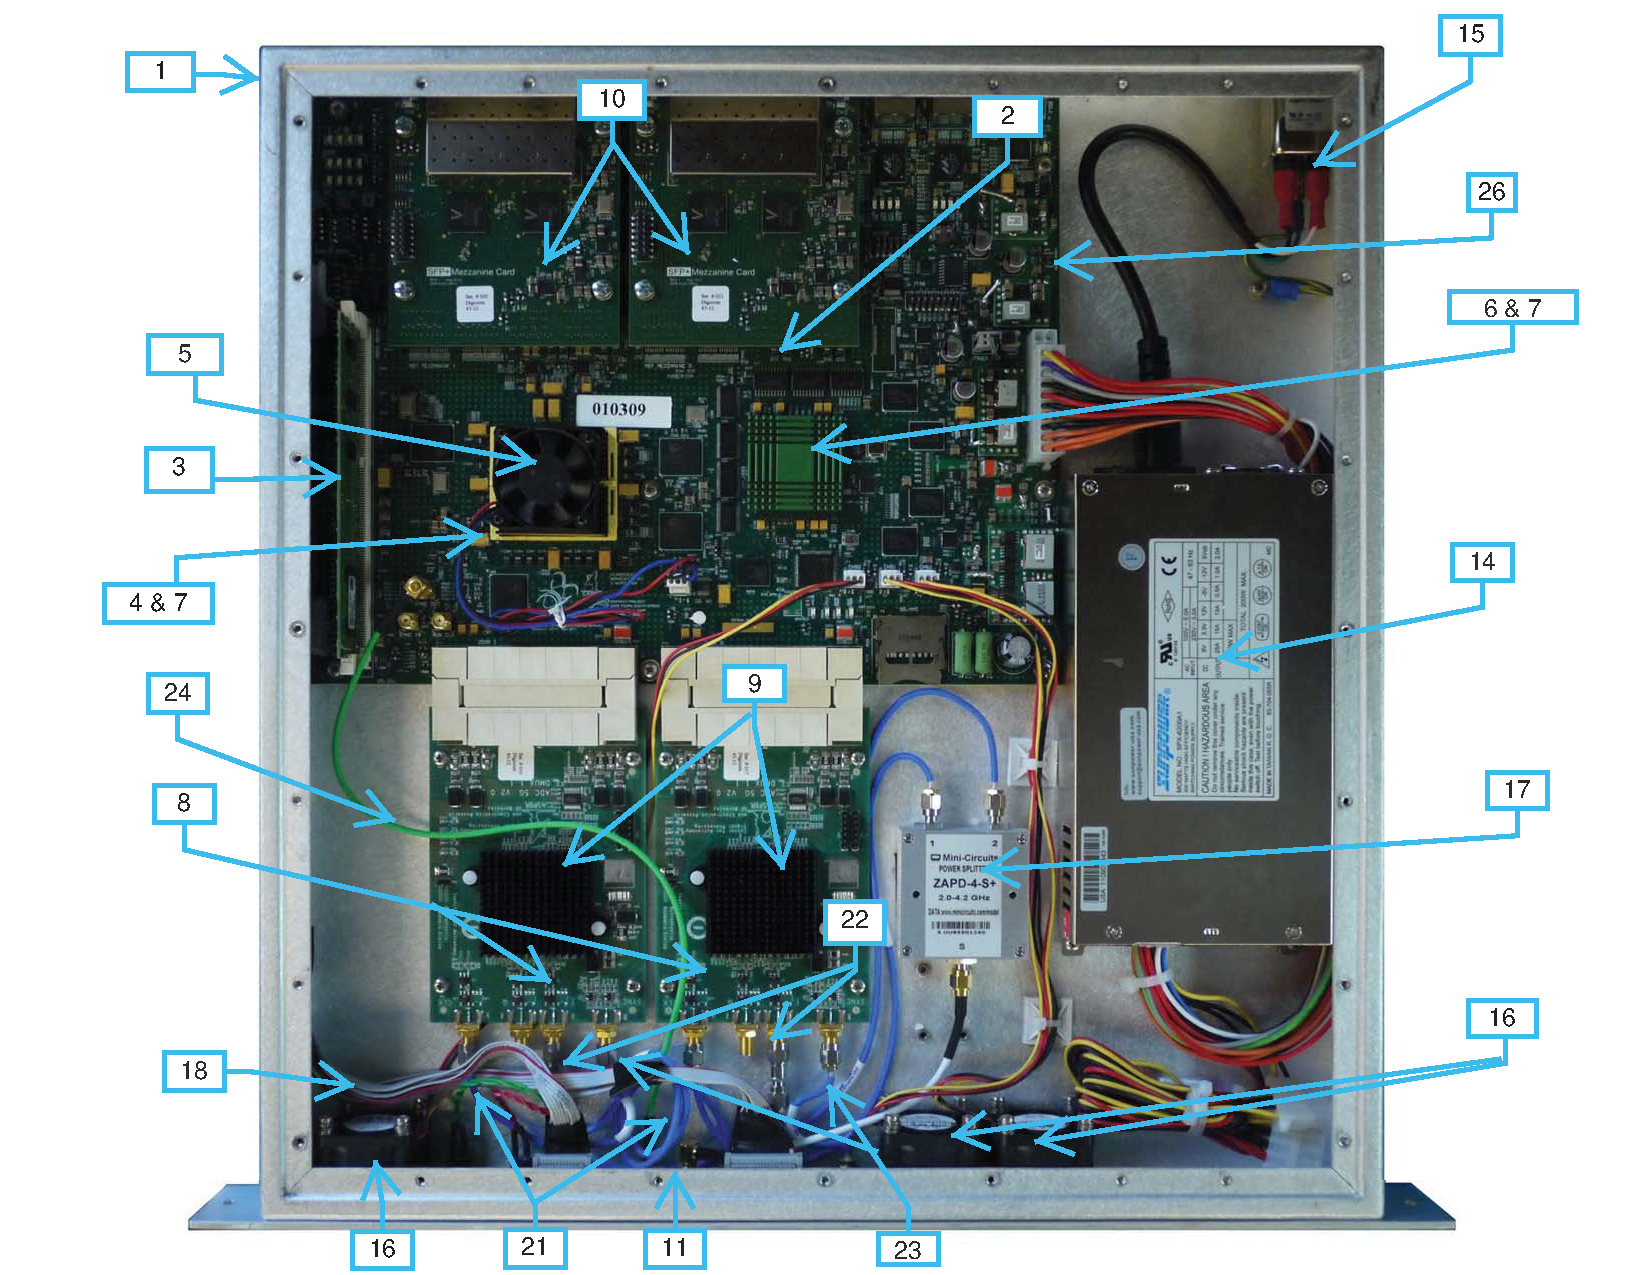
\includepdf[pages=-]{ROACH2-ASSYv4.pdf}

\end{document}
